\chapter{\textcolor{black}{Foundations of Generative Models and Evaluation metrics}}\label{ch: generative_models}
\thispagestyle{plain}
The content of this chapter is based almost entirely on the current state of the art. The contribution of the author of this thesis is the introduction of the Traffic signs classification accuracy metric. This is presented at the end of the chapter and proposed in:
\begin{quotation}
\noindent \textit{\textbf{\large C-SPIC: Class-Specific Semantic-Preserving Image Coding with Residual Enhancement for Accurate Object Recovery}}\\
\textit{Francesco Pezone, Osman Musa, Giuseppe Caire, Sergio Barbarossa}
\end{quotation}

\section{Introduction}
Generative models represent a powerful class of \gls{ml} algorithms. Their capability to learn the underlying data distribution and to reconstruct or generate new data samples has made them some of the most utilized tools in \gls{ml}.

Since the introduction of early statistical methods like \textit{Restricted Boltzmann Machine} and \textit{Gaussian Mixture Model} \cite{Salakhutdinov2015surveyGenMod}, the field of generative models has undergone significant transformations. As task complexity increased, these initial approaches became inadequate for capturing the complexity of modern data distributions. While early models were effective in generating convincing images on simple datasets such as MNIST \cite{Lecun2010mnist}, which contains handwritten digits and the NORB dataset \cite{LeCun2004NORBdataset}, featuring small black-and-white toy images, more complex datasets like CIFAR10 and CIFAR100 \cite{Krizhevsky2009CIFAR} or ImageNet \cite{Russakovsky2015ImageNet} highlighted their limitations.

The first important breakthrough in the field of \gls{ml} came in 2012 with the introduction of AlexNet \cite{Krizhevsky2012Alexnet}. This architecture completely revolutionized the field by showing the incredible power of \glspl{dnn}, and more specifically of deep \gls{cnn}, in capturing complex details in the data distribution. AlexNet also popularized GPU acceleration for model training, the ReLU activation function \cite{Nair2010ReLU} and dropout for regularization \cite{Hinton2012dropout}, fundamentally changing the approach to \gls{ml}.

Shortly afterwards, architectures like the \gls{ae} \cite{Rumelhart1986Autoencoder} and the \gls{unet} \cite{Ronneberger2015Unet} were developed. While AlexNet was designed for classification tasks, these new architectures were proposed to work towards domains more closely related to generative models. The \gls{ae} was designed to capture a simplified latent representation of images and reconstruct them, while the \gls{unet} was specifically designed for \gls{sseg} tasks.

Building upon these architectures, a wide variety of new models have been developed in recent years. The \gls{ae} inspired the development of \glspl{vae} \cite{Kingma2014VAE, Kingma2019VAE}, incorporating probabilistic frameworks into the \gls{ae} structure. Then the introduction of \glspl{gan} \cite{goodfellow2014generative} introduced a new training paradigm based on two adversarial networks being optimized in a game theory scenario. Further advancements led to vector-quantized versions, such as the \gls{vqvae} \cite{Oord2017VQ-VAE} and the \gls{vqgan} \cite{Esser2O21Taming}. More recently, the family of \gls{ddpm} \cite{Ho2020ddpm} has gained significant attention for their innovative multistep approach in generating new data samples. These models have dramatically improved data generation quality,  enabling the generation of highly detailed images from simple text descriptions.

This chapter explores these models in parallel to some of the most important building blocks commonly used across many different architectures.  The \gls{ae}, \gls{unet}, \gls{resblock}, \gls{vae} and the \textit{Attention Mechanism} are fundamental components in a majority of the architectures discussed in this thesis. Understanding them is crucial before moving on to more complex architectures.

In \sref{sec: GM gan} the \gls{gan} architecture is discussed and in \sref{sec: GM vq-vae} the vector-quantized versions, such as the \gls{vqvae} and \gls{vqgan}, are introduced highlighting the advantages of vector quantization. Finally, the \gls{ddpm} models are analyzed, covering the techniques and concepts most relevant to this work.

In addition to exploring these generative models, this chapter also introduces the evaluation metrics and loss functions employed throughout this work. Selecting appropriate metrics and losses is crucial for designing, training, and assessing the performance of the models. The last section provides a comprehensive overview of both classic evaluation metrics, commonly used in image compression and reconstruction tasks, and semantic-relevant metrics, which evaluate the preservation of semantic information in the data. These metrics are particularly important in the context of \gls{sc} frameworks.

\section{The Building Blocks}\label{sec: GM unet}
This section is devoted to some of the most fundamental building blocks in the design of many generative models: the \gls{ae}, the \gls{unet}, the \gls{vae} and the \textit{Attention Mechanism}. The first three refer to complete architectures that serve as the starting points for the more complex models used in this thesis. They provide the necessary structures for encoding, decoding, and transforming data across different latent representation. The last one, the Attention Mechanism, is instead an important component widely used in modern \gls{ml}. This component is used to improve the performance of other models by allowing them to focus on specific parts of the data. Unlike classical convolutional layers, the attention mechanism can connect parts of the data that are spatially far apart.

\subsection{Autoencoder}

Proposed in \cite{Rumelhart1986Autoencoder}, the \acrlong{ae} is a type of neural network designed to reconstruct its input by learning an efficient representation of the data in an unsupervised way.\\
\glspl{ae} can vary greatly in complexity, ranging from \gls{ae} based on convolution operations to \gls{fc} layers. The one constant is the underlying structure composed of two main parts:

\begin{itemize}
    \item \textbf{Encoder:} The encoder network is the interface between the input data $\x$ and the latent representation $\z$. Its goal is to reduce the complexity of the initial data by preserving only the most relevant features.  

    \item \textbf{Decoder:} The decoder network is responsible for reconstructing the input data $\x$ from the latent representation $\z$. This network typically mirrors the encoder in structure but reverses the dimensionality reduction layers to progressively up-scale the latent tensor back to the original input size. The decoder's goal is to produce an output that is as close as possible to the original input by minimizing the reconstruction error.
\end{itemize}

By altering the type of encoder and decoder, different results can be achieved by an \gls{ae}. For example, if the encoder and decoder are composed of a series of \gls{fc} layers without nonlinear layers, then the \gls{ae} achieves the same latent representation as the \textit{Principal Component Analysis}, as shown in \cite{Plaut2018FromPS}.\\
Other powerful ways to design the \gls{ae} involve the use of \glspl{dnn} and convolutional layers. These more advanced architectures allow the capture of more complex patterns in the input data and provide the necessary power to handle input domains of increased complexity.\\
In general, \glspl{ae} are trained using some form of reconstruction loss to ensure that the reconstructed output resembles the input data. Examples of these reconstruction losses include \gls{l2} or \gls{l1}. However, for specific needs and advanced tasks, other forms of loss can be used to better approximate non-trivial data distributions.

\subsection{U-Net Architecture}\label{sec: GM unet}
\begin{figure}[!t]
    \centering
    \includegraphics[width=0.5\textwidth]{Figures/Generative_models/resblock_classico.pdf}
    \captionsetup{width=.8\linewidth}
    \caption[\acrshort{resblock} architecture scheme]{Architectural diagram of the \gls{resblock}. The residual connection is represented by the line that goes from $h_{l-1}$ to the sum symbol.}
    \label{fig: GM resblock}
\end{figure}
The increasing complexity of both tasks and \gls{nn} depth presented various challenges to the classical \gls{ae}. \gls{sseg} tasks, for instance, highlighted the limitations of the bottleneck structure of the \gls{ae}, which often caused the loss of fine detail. In fact, the down-scaled latent space was insufficient for guaranteeing a good reconstruction of an output data with the same resolution as the input, since it did not effectively preserve spatial information. Another challenge was related to adapting the training process to the increased depth of \glspl{nn}. Since these networks are usually trained through backpropagation, the deeper the network, the longer the gradient has to "travel" backward. This results in the so-called problem of vanishing gradient \cite{Pascanu2013vanishGrad}, where the gradient becomes too small for effective training. 

To overcome these problems, the \gls{unet} was introduced in \cite{Ronneberger2015Unet}. Its structure is based on the \gls{ae} architecture, with the same encoder-decoder mirrored structure, and with some additional layers in between the encoder and decoder. These additional layers are called bottleneck layers and are used to further process the latent representation before it is handled by the decoder. However, the most important innovations in the \gls{unet} architecture consist in the extensive use of \glspl{resblock} and the introduction of the \textit{skip connections}. 

\begin{itemize}[label={}]
    \item{\textbf{ResBlock}:} Introduced by He et al. in \cite{He2016ResBlock}, not specifically for \glspl{unet}, this block was designed to help overcome the problem of the vanishing gradient. Before its introduction, the main approach was to use a long series of alternating convolutional layers, some nonlinear activation functions, and normalization, with a noticeable example being AlexNet \cite{Krizhevsky2012Alexnet}. He et al. proposed a new way of designing a network. Instead of a long uninterrupted sequence of convolution, activation, and normalization layers, the idea was to create a block, the \gls{resblock}, with a particular characteristic. 
    Every block is composed of a series of convolution, activation, and normalization layers that are repeated a given number of times, generally twice. The main difference lies in the introduction of the \textit{residual connection}. Every time a hidden layer $h_i$ encounters a \gls{resblock}, it is processed by the layers of the \gls{resblock} and at the end, the input is summed with the output, as illustrated in \fref{fig: GM resblock}.\\
    The role of the residual connection is to reduce the risk of degradation by providing shortcuts for the propagation of critical information. At the same time, during backpropagation their role is to split the gradient: one part is directed inside the block, allowing the parameters to be updated, while the other is copied at the other end, mitigating the vanishing gradient problem.
    
    \item{\textbf{Skip Connections}:} The innovation introduced by the \gls{unet} is the concept of skip connections. In fact, while the residual connection is adopted locally between a few layers, the skip connection works on a completely different scale. 
    \begin{figure}[!t]
        \centering
        \includegraphics[width=0.8\textwidth]{Figures/Generative_models/u-net-architecture.png}
        \captionsetup{width=.8\linewidth}
        \caption[\acrshort{unet} architecture scheme]{Architectural diagram of the \gls{unet} as proposed in \cite{Ronneberger2015Unet}. The encoder and decoder are linked via the skip connections represented in gray.}
        \label{fig: GM unet}
    \end{figure}
    As illustrated in \fref{fig: GM unet}, the skip connections link corresponding layers between the encoder and decoder. This has a double advantage: (i) during backpropagation, they allow the gradient to flow from the decoder to the encoder unchanged, avoiding the vanishing gradient, and (ii) during the forward process, they help preserve details. \\
    With skip connections, the model can reuse features extracted in the encoder at different resolutions even at the decoder. This enhances the ability of the \gls{unet} to generate detailed and accurate outputs. The decoder can access features processed both through the bottleneck but also features that are at the same level of detail. This is particularly important in tasks where preserving spatial information is critical, such as \gls{sseg} and \gls{sr}.
\end{itemize}

The main factor distinguishing the \gls{unet} from the \gls{ae} is the presence or absence of skip connections.\\
Even though skip connections encourage the preservation of detail, this does not automatically mean that the \gls{unet} is always better than the \gls{ae}. One of the advantages of using a \gls{unet} is its ability to preserve fine details, while one of its drawbacks is its shortcomings in data compression. In fact, while an \gls{ae} only requires the latent representation $\z$ to reconstruct the output, this would not be sufficient for a \gls{unet}, as all the intermediate skip connections would also have to be used. The choice of an \gls{ae} over a \gls{unet} is therefore strongly dependent on the task.\\

While skip connections are specific to \glspl{unet}, \glspl{resblock} are a tool widely used in \gls{ml}. They are not specifically designed for \glspl{unet}; an \gls{ae} can be designed to include \glspl{resblock} as well. The advantages of \glspl{resblock} go beyond countering the vanishing gradient. They also offer a practical and simpler way to design a model. In fact, a model based on \glspl{resblock} can be easily modified to achieve better control over the output.\\
The scheme illustrated before in \fref{fig: GM resblock} represents only the base structure of a \gls{resblock}. However, by modifying its structure it is possible to condition its behavior on external factors. For example, in some cases it might be useful to introduce some form of time dependency. This can be easily achieved by modifying the \gls{resblock} architecture, as depicted in \fref{fig: GM resblock with time}, where the time conditioning is introduced by a linear application.
\begin{figure}[t]
    \centering
    \includegraphics[width=0.5\textwidth]{Figures/Generative_models/resblock_time_conditioning.pdf}
    \caption[\acrshort{resblock} architecture scheme with time conditioning]{Architectural diagram of the \gls{resblock} conditioned on the time $t$. The value $t$ is mapped to an higher dimensional space via the \gls{pe} before being inserted in the \gls{resblock}.}
    \label{fig: GM resblock with time}
\end{figure}
The first step involves mapping the time $t$ into a high-dimensional space that can be easily interpreted by the \gls{nn}. This is done via the so-called \gls{pe}, a technique developed for the Transformer architecture \cite{Vaswani2017AttentionIsAllYouNeed}. The idea is to map the value $t$ into a fixed or learnable higher-dimensional space, the $PE(t)$ vector, that can then be further transformed, for example via a \gls{fc} layer. This final transformation is now inserted in the middle of the \gls{resblock} and this conditioning will allow the model to learn the effects of time and reflect them in the result.\\
Another interesting example is the case where the performances are influenced by the \gls{ssm}. In this case, it is possible to modify the structure of the \gls{resblock} by substituting the classical normalization layer with the \gls{spade} layer introduced by Park et al. in \cite{Park2019SPADE}. They proposed a variation of the classical Batch Normalization layer \cite{Ioffe2015Batchnorm} that uses the information extracted from the \gls{ssm} to condition the normalization.

\begin{figure}[!t]
    \centering
    \includegraphics[width=0.4\textwidth]{Figures/Generative_models/resblock_spade.pdf}
    \hfill
    \raisebox{0\height}{\includegraphics[width=0.59\textwidth]{Figures/Generative_models/Spade_batchnorm.png}}
    \caption[\acrshort{spade} layer and \acrshort{resblock} architecture scheme]{On the left, the architectural diagram of the \acrshort{resblock} proposed in \cite{Park2019SPADE} that introduces \acrshort{spade}, a normalization technique able to condition on the \acrshort{ssm}. On the right, the \acrshort{spade} architecture is compared with batch normalization. The parameters $\gamma$ and $\beta$ are now learned as functions of the input \gls{ssm}.}
    \label{fig: GM resblock spade}
\end{figure}

More specifically, the main idea of their new \gls{spade} layer is depicted in the right scheme in \fref{fig: GM resblock spade}. In Batch Normalization, the re-scaling is achieved through two learnable parameters, $\gamma$ and $\beta$. These parameters are used to perform the linear transformation $BatchNorm(\h) = \gamma \h + \beta$ of the hidden variable $\h$. The intuition behind the \gls{spade} layer is to learn these parameters as a function of the \gls{ssm}. This is done as follows:
\begin{equation}
    SPADE(\h,\s) = f(\s) \h + g(\s),
\end{equation}
where $f$ and $g$ represent the \glspl{cnn} responsible for transforming the \gls{ssm} $\s$. The new $\gamma=f(\s)$ and $\beta=g(\s)$, while being used to normalize are also able to enforce the desired structure of the \gls{ssm} on the output. The structure of the new \gls{ssm} conditioned \gls{resblock} is shown on the left side of \fref{fig: GM resblock spade}. 

An important consideration has to be made on the effects of these conditioning. In fact, it is fundamental to introduce these modified \glspl{resblock} only in those parts of the \gls{unet} where their impact is maximized. To condition the feature extraction is good practice to condition the encoder blocks of the \gls{unet}. On the other hand, if the final purpose is to influence the output result the best option is to condition in the bottleneck and the decoder. For example, when the \gls{ssm} needs to be enforced on the output the modified \gls{resblock} in \fref{fig: GM resblock spade} should be placed in the bottleneck and decoder. Instead, in some other cases the conditioning variable is relevant throughout the whole process and all the \glspl{resblock} would be influenced. This is the case with the time conditioning.
 
\subsection{Variational Autoencoders}\label{sec: GM vae}
\begin{figure}[!h]
    \centering
    \includegraphics[width=0.7\textwidth]{Figures/Generative_models/Schema_vae.pdf}
    \caption[\acrshort{vae} architecture scheme]{Overview of the \acrshort{vae} architecture. The latent tensor is obtained as $\z=\boldsymbol{\mu} + \boldsymbol{\sigma} \odot \boldsymbol{\epsilon}$ via the reparameterization trick by selecting a random value $\bepsilon \sim \N(0, I)$.}
    \label{fig: GM schema_vae}
\end{figure}
A \gls{vae} \cite{Kingma2014VAE, Kingma2019VAE} extends the concept of classical \glspl{ae} by introducing a probabilistic framework to the encoding and decoding processes, \fref{fig: GM schema_vae}. Unlike the \glspl{ae}, that uses a deterministic approach, the  \glspl{vae} consider the encoding process as probabilistic. The data $\x$ is associated to a probability distribution $q(\x)$ that allow better generating capabilities. However, the direct use of $q(\x)$ to generate data is unfeasible because of its complexity in being directly estimated. To overcome this issue the \gls{vae} is designed to work with two simpler probability distributions: $q(\x|\z)$ and $q(\z|\x)$. They represent the core processes of encoding the data $\x$ to a latent representation $\z$ and then retrieving the original data back. Unfortunately, even if simpler than the $q(\x)$, these two distributions are still very complex and impossible to know exactly. This problem can be tackled by approximating them with the help of \glspl{dnn}.

Instead of dealing with $q(\z|\x)$ and $q(\x|\z)$, it is possible to consider the two approximating distributions $q_\phi(\z|\x)$ and $p_\theta(\x|\z)$ parameterized by two \gls{dnn} with parameters $\phi$ and $\theta$, respectively. Moreover, to further reduce the complexity, these approximations are usually forced to be Gaussian distributions.  This choice drastically reduces the complexity by shifting the problem from estimating an unknown probability distribution to estimating the mean and variance of a Gaussian distribution.\\

The key objective of a \gls{vae} is to maximize the likelihood of the observed data $q(\x) = \int q(\x|\z) q(\z) d\z$. However, directly maximizing this term is intractable due to the complexity of computing this value. To overcome this, \gls{vae} optimize the \gls{elbo}, which provides a tractable lower bound on the likelihood:

\begin{equation} \log q(\x) \geq ELBO(\x) =  \underbrace{\mathbb{E}_{q_{\phi}(\z|\x)} \left[ \log p_\theta(\x|\z) \right]}_{\text{Reconstruction Term}} - \underbrace{\mathcal{D}_{\text{KL}}(q_\phi(\z|\x) \parallel q(\z))}_{\text{Regularization Term}}. \label{eq: GM vae elbo_summarized} \end{equation}

The ELBO consists of two terms:

\begin{itemize} 
    \item \textbf{Reconstruction Term:} Encourages the decoder $p_\theta(\x|\z)$ to accurately reconstruct the input data from the latent representation. 
    \item \textbf{Regularization Term:} Encourages the encoder $q_\phi(\z|\x)$ to be close to the prior distribution $q(\z)$, typically chosen as a standard normal distribution as well. 
\end{itemize}

The training idea is to use the encoding network $q_\phi(\z|\x)$ to estimate the mean $\boldsymbol{\mu}$ and standard deviation $\boldsymbol{\sigma}$ of the true $q(\z|\x)$ and use them to sample the latent variable $\z$. This value is then used to reconstruct the data $\x$ with the decoding network $p_\theta(\x|\z)$. However, during backpropagation it would be better if the gradient could flow backward through the network and update the weights. Unfortunately, the sampling operation of $\z$ introduces a non-differentiability, which prevents backpropagation from updating the encoder weights.

To solve this problem, Kingma and Welling introduced the \textit{Reparameterization Trick} in the context of \gls{vae} \cite{Kingma2014VAE}. Instead of sampling $\z$ directly from $q_\phi(\z|\x)$, it is sampled with the help of an auxiliary variable $\boldsymbol{\epsilon} \sim \mathcal{N}(0, \mathbf{I})$ obtaining: 
\begin{equation}
    \z = \boldsymbol{\mu} + \boldsymbol{\sigma} \odot \boldsymbol{\epsilon}, 
\label{eq: GM vae z_reparametrized_summarized} 
\end{equation}

where $\boldsymbol{\mu}$ and $\boldsymbol{\sigma}$ are the mean and standard deviation output by the encoder network, and $\odot$ denotes element-wise multiplication.

The advantage is that the sampling process is now differentiable in $\boldsymbol{\mu}$ and $\boldsymbol{\sigma}$ and the gradient can flow back through the encoder to train the model. All the stochasticity is confined and depends on $\bepsilon$. It is important to notice that the system is still not differentiable with respect to $\bepsilon$, but this is not relevant in the optimization of the network.

The loss function used to train the \gls{vae} is derived from the negative ELBO as follows:
\begin{align}
    - \text{ELBO}(\x_i) \approx \Loss(\x_i ) &=  \frac{1}{L} \sum_{l=1}^{L} \frac{1}{2\sigma^2} \left( \left\| \x_i - \hat{\x}_{i,l} \right\|^2 \right) + \mathcal{D}_{\text{KL}}(q_\phi(\z|\x_i) \parallel q(\z))  \label{eq: GM vae loss_function_extended}\\
    &= \Loss_{\text{rec}}(\x_i) + \Loss_{\text{KL}}(\x_i ) \equiv \Loss_{\text{rec}} + \Loss_{\text{KL}} ,
\end{align}
where $\x_i$ is the $i$-th input data and $\hat{\x}_{i,l} = D_\theta(\z_{i,l})$ is the output of the decoder network.\\

Even if this loss function can already allow the \gls{vae} to generate good samples, it is good practice, as introduced in \cite{Higgins2016betaVAE}, to re-scale the different terms by a factor $\beta$. Also known as $\beta$-\gls{vae}, this new approach uses the following loss function:
\begin{equation}
    \Loss = \Loss_{\text{rec}} + \beta \Loss_{\text{KL}}.
\label{eq: GM vae beta_vae}
\end{equation}

The advantages are numerous, in fact the $\beta$-\gls{vae} is able to control the trade-off between the reconstruction and the regularization term, allowing the user to decide which one to prioritize. Different values of $\beta$ can lead to different outputs:
\begin{itemize}
    \item $\beta=1$: the classical \gls{vae} discussed until now
    \item $\beta>1$: prioritizes the regularization term, encouraging the latent representations to be more disentangled, meaning that individual dimensions of the latent space capture more distinct and interpretable factors. For example one component might focus on the shape of the eyes and one on the color. However, this can come at the cost of reconstruction accuracy.
    \item $\beta<1$: prioritizes the reconstruction term, leading to better reconstructions but poorer disentanglement of the latent factors. In this case any component might influence more than one factor.
\end{itemize}

By adjusting $\beta$, the trade-off between reconstruction fidelity and latent space regularization can be tweaked according to specific requirements. This approach is beneficial for applications where the interpretability of the latent space is crucial, or when the goal is to enhance the generative capabilities of the model.

\subsection{Attention Mechanism}\label{sec: GM attention}

The attention mechanism is a fundamental component in modern machine learning models, particularly in tasks involving sequence data, such as natural language processing and time series analysis. Introduced in \cite{Bahdanau2014Attention} and popularized by the Transformer architecture proposed in \cite{Vaswani2017AttentionIsAllYouNeed}, the attention mechanism allows the model to focus on specific parts of the input data. 

The core idea of the attention mechanism is to compute a weighted sum of the input elements, where the weights are dynamically determined based on the relevance of each element to the current task. This approach enables the model to selectively pay attention, \textit{attend}, to important information while ignoring non-relevant parts, leading to improved performance in tasks requiring context awareness.\\
The attention mechanism works by assigning three main vector representations to each input element: the query ($\mathbf{Q}$), the key ($\mathbf{K}$), and the value ($\mathbf{V}$). Drawing from concepts in information retrieval, the query $\mathbf{Q}$ identifies the information being sought, while the key $\mathbf{K}$ encodes the relevant features of the data that could match the query. The query and keys are processed together through a function that measures their compatibility, generating a score that indicates how well they align. This attention score ($\text{A}_{\text{score}}$) highlights which keys are most relevant to the query. The value $\mathbf{V}$ contains the actual data associated with each key and is retrieved based on the attention score, with higher scores giving more importance to the corresponding values.

The simplest form of attention is the so-called \textit{scaled dot-product attention}. In this version, the attention score is computed as the dot product of the query and key vectors, scaled by the inverse of the square root of the dimensionality of the key vectors, $d_k$. Then, a non-linearity is applied via the softmax function and these weights are then used to compute a weighted sum of the value vectors. The formula is:

\begin{equation}
\text{Attention}(\mathbf{Q}, \mathbf{K}, \mathbf{V}) = \text{A}_{\text{score}} \mathbf{V} = \text{softmax}\left(\frac{\mathbf{Q} \mathbf{K}^T}{\sqrt{d_k}}\right) \mathbf{V}
\label{eq: GM attention single head}
\end{equation}

The use of the attention score allows the model to dynamically weigh the importance of different input elements. The weights are directly linked to the query and key and the attention score adapt better than classical linear transformations to complex tasks.\\
Similar to the information retrieval scenario, every attention layer correspond to a request of information to the data. A single question is in general not necessary to extract multiple information. For this reason, a more commonly used practice is to use the \textit{Multi-Head Attention mechanism}. This mechanism consists of multiple attention mechanisms (or heads) running in parallel. This is used to capture different types of relationships in the data, where each head has its own set of query, key, and value matrices. The outputs from each head are then concatenated and linearly transformed to produce the final output:
\begin{equation}
\text{multi-head}(\mathbf{Q}, \mathbf{K}, \mathbf{V}) = \text{Concat}(\text{head}_1, \text{head}_2, \dots, \text{head}_h) \mathbf{W}^O,
\label{eq: GM attention multi head}
\end{equation}
where each attention head is computed as:
\begin{equation}
\text{head}_i = \text{Attention}(\mathbf{Q} \mathbf{W}^Q_i, \mathbf{K} \mathbf{W}^K_i, \mathbf{V} \mathbf{W}^V_i),
\end{equation}
with \(\mathbf{W}^Q_i\), \(\mathbf{W}^K_i\), \(\mathbf{W}^V_i\), and \(\mathbf{W}^O\) as learnable weight matrices specific to each attention head and the output linear transformation.\\

This mechanism can be used in many fields, from computer vision to natural language processing. By changing the input data and the query, key, and value structure, the attention mechanism can be adapted to specific tasks, resulting in different types of attention. One example is \textit{Self-Attention}, where the query, key, and value vectors are all derived from the same input. This allows each element to attend to all other elements. If the query is derived from a different input than the key and value, the attention mechanism is called \textit{Cross-Attention}. This is another possible technique used to condition the reconstruction on an external input. In Stable Diffusion \cite{rombach2022high}, cross-attention is widely used to condition the output on text input. In this case, the query is derived from the latent representation, while the key and value are obtained from the conditioning text. This allows the model to focus on relevant aspects of the text when generating the image, guiding the reconstruction process based on the given input.





\begin{comment}
\section{Variational Autoencoders}\label{sec: GM vae}
A \gls{vae} \cite{Kingma2014VAE, Kingma2019VAE} is a type of generative model that generalizes the concept of classical \gls{ae} by introducing a probabilistic approach to the encoding and decoding processes.
\begin{figure}[!h]
    \centering
    \includegraphics[width=0.7\textwidth]{Figures/Generative_models/Schema_vae.png}
    \caption[\acrshort{vae} architecture scheme]{Variational Autoencoder Architecture with latent space $\z$ and encoder-decoder.}
    \label{fig: GM schema_vae}
\end{figure}
\fref{fig: GM schema_vae} represents the general idea behind a \gls{vae}. Unlike a classical \gls{ae}, the \gls{vae} uses a probabilistic approach. It consider the probability distributions associated with $\x$ and $\z$, and not only a deterministic transformation.\\
The first important step is to define some of the probability distributions that will be used in the following sections:
\begin{itemize}
    \item $q(\x)$: the true unknown data distribution
    \item $q(\z)$: the prior distribution of the latent space, usually a simple distribution like a normal distribution
    \item $q(\z|\x)$: the posterior distribution of the latent variable given the data, which the encoder network tries to approximate
    \item $q(\x|\z)$: the likelihood of the data given the latent variable, corresponding to the distribution the decoder network tries to approximate 
\end{itemize}
The most interesting distribution among these four is $q(\x)$. Knowing it would mean that sampling from the true data distribution is solved and it would be possible to generate perfect data. This is unfortunately not realistic due to the complexity of such a distribution.\\
The idea of the \gls{vae} is to go around this problem by focusing on the two conditional distributions $q(\x|\z)$ and $q(\z|\x)$. They represent the core processes of encoding the data $\x$ to a latent representation $\z$ and then retrieving the original data back and working with them simpler than working with the data distribution $q(\x)$. Unfortunately, even these distributions are very complex and impossible to know exactly. The only possible approach to overcome this issue is to approximate them. A possible way is by using the generalization power of \gls{dnn}.\\
Instead of dealing with $q(\z|\x)$ and $q(\x|\z)$, it is possible to consider two approximating distributions:
\begin{itemize}
    \item $q_\phi(\z|\x)$, which is represented by the \textbf{encoder} network and tries to approximate $q(\z|\x)$
    \item $p_\theta(\x|\z)$, which is represented by the \textbf{decoder} network and tries to approximate $q(\x|\z)$
\end{itemize} 
The advantage of using these approximations lies in the use of the \gls{dnn} structure that can be used to estimate their parameters via backpropagation.
Even if \gls{dnn} are very powerful understanding the real unknown distributions would still be too complicated. To further reduce the complexity these approximations are often forced to be Gaussian distributions. This approach drastically reduces the complexity by shifting the problem of estimating an unknown probability distribution to estimating the mean and variance of a Gaussian distribution.

\subsection{Evidence Lower Bound (ELBO)}
After defining the main structure of the desired probability distributions, it is important to understand what a \gls{vae} is trying to optimize.\\
As mentioned before, the main goal of a \gls{vae} is to maximize the likelihood of the observed data $q(\x)$, which is equivalent to minimizing the negative log-likelihood of the same distribution. However this cannot be done directly due to the intractability of directly computing the marginal likelihood $q(\x)$. Even in this case it is necessary to introduce some approximations to make the problem tractable. \\
Starting from the log-likelihood $\log q(\x)$ and multiplying it by $\int q_\phi(\z|\x) dz = 1$ it is possible to obtain:
\begin{equation}
    \log q(\x) = \int \log q(\x)  q_\phi(\z|\x) dz  = \mathbb{E}_{q_\phi(\z|\x)} \left[ \log q(\x) \right].
\end{equation}
This is still not enough and the problem remains that the expected value is evaluated for the unknown distribution $q(\x)$. Thanks to Bayes' theorem, it is possible to , removing this dependence and rewrite the previous equation as:
\begin{align}
    \log q(\x) &= \mathbb{E}_{q_\phi(\z|\x)} \left[ \log q(\x) \right] = \mathbb{E}_{q_\phi(\z|\x)} \left[ \log \frac{q(\x,\z)}{q(\z|\x)} \right] \\
    &= \underbrace{\mathbb{E}_{q_\phi(\z|\x)} \left[ \log \frac{q(\x,\z)}{q_\phi(\z|\x)} \right]}_{\text{ELBO}} + \underbrace{\mathbb{E}_{q_\phi(\z|\x)} \left[ \log \frac{q_\phi(\z|\x)}{q(\z|\x)} \right]}_{\mathcal{D}_{\text{KL}}\left( q_\phi(\z|\x) \| q(\z|\x) \right)}.
\end{align}
where multiplication and division by $q_\phi(\z|\x)$ were used as long as the properties of the logarithms. \\
The first term corresponds to the so called \gls{elbo}, while the last term is the Kullback-Leibler divergence.
The $\mathcal{D}_{\text{KL}}$ is evaluated between the approximate posterior $q_\phi(\z|\x)$ and the real $p(\z|\x)$. This value is an always positive term measuring how much the approximate posterior deviates from the real one.\\
The meaning of the equation can be understood by rearranging the terms and isolating the $\mathcal{D}_{\text{KL}}$.  This can be graphically be summarized by the following schema.
\begin{figure}[!h]
    \centering
    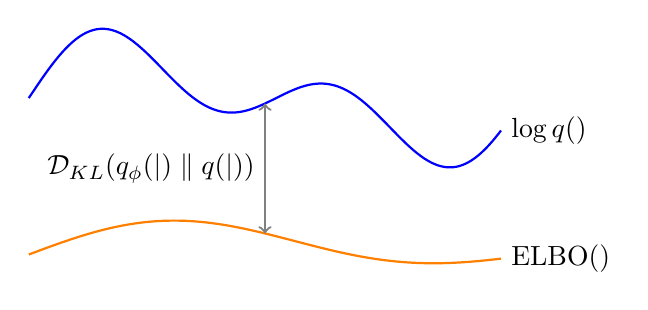
\begin{tikzpicture}
        % Draw the log p(\x) curve with increased complexity
        \draw[blue, thick, domain=0:6, samples=200] plot (\x, {0.5*sin(\x r) + 0.5*sin(2*\x r) + 3}) node[right, black] {$\log q(\x)$};
        
        % Draw the ELBO curve with smoother shape
        \draw[orange, thick, domain=0:6, samples=200] plot (\x, {0.25*sin(\x r + 1) + 0.25*sin(0.5*\x r + 2) + 1}) node[right, black] {ELBO$(\x)$};
        
        % Draw the vertical distance with an arrow
        \draw[gray, thick,<->] (3, {0.5*sin(3 r) + 0.5*sin(2*3 r) + 3}) -- (3, {0.25*sin(3 r + 1) + 0.25*sin(0.5*3 r + 2) + 1}) node[midway, left, black] {$\mathcal{D}_{\text{KL}}(q_\phi(\z|\x) \parallel q(\z|\x))$};
    \end{tikzpicture}
\end{figure}
It is possible to interpret the $\mathcal{D}_{\text{KL}}$ as the distance between the $\log q(\x)$ and the \gls{elbo}. The $\log q(\x)$ is also called the \textit{evidence}.  Since the $\mathcal{D}_{\text{KL}}$ is always positive, the following relation holds:
\begin{equation}
    \log q(\x) \geq \text{ELBO}(\x),
\end{equation}
which explains the origin of the name \textit{evidence lower bound}.\\
Maximizing $\log q(\x)$ does not require anymore knowing $q(\x)$, but can now be achieved by maximizing the \gls{elbo}. This approach has multiple benefits: (i) it deals with simpler probability distributions, (ii) maximizing it is equivalent to maximizing $\log q(\x)$, and (iii) maximizing it leads to a minimization of the $\mathcal{D}_{\text{KL}}$, forcing the \gls{elbo} to better approximate the $\log q(\x)$.\\
This graphical interpretation helped in better understanding what has to be optimized but did not solve the problem. The \gls{elbo} still contains the unknown $q(\x,\z)$. To address this, it is necessary to rewrite the \gls{elbo} in a more tractable way by using Bayes' theorem and the properties of the logarithm as follows:
\begin{align}
    \log q(\x) \geq \text{ELBO}(\x) &= \mathbb{E}_{q_\phi(\z|\x)} \left[ \log \frac{q(\x,\z)}{q_\phi(\z|\x)} \right] = \mathbb{E_{q_\phi(\z|\x)}} \left[ \log \frac{q(\x|\z)q(\z)}{q_\phi(\z|\x)} \right] \\  
    &= \mathbb{E_{q_\phi(\z|\x)}} \left[ \log q(\x|\z) \right] + \mathbb{E_{q_\phi(\z|\x)}} \left[ \log \frac{q(\z)}{q_\phi(\z|\x)} \right] \\
    &= \mathbb{E_{q_\phi(\z|\x)}} \left[ \log p_\theta(\x|\z) \right] - \mathcal{D}_{\text{KL}}(q_\phi(\z|\x) \parallel q(\z)),
\label{eq: GM vae elbo}
\end{align}
where in the last equation, the real $q(\x|\z)$ was substituted with the approximate $p_\theta(\x|\z)$, and the definition of KL divergence was applied.\\
At this point, \eref{eq: GM vae elbo} is composed of all known quantities:
\begin{itemize}
    \item The first term refers to the \textit{reconstruction term}, which encourages the decoder $p_\theta(\x|\z)$, Gaussian by design, to accurately reconstruct the input data.
    \item The second term is the \textit{regularization term}, which ensures that the encoder $q_\phi(\z|\x)$, Gaussian by design, is as close as possible to the prior $q(\z)$, usually a standard normal distribution.
\end{itemize}

Both terms can now be optimized using backpropagation since all the unknown distributions have been substituted by their respective approximations. \\
The result is that the model learns how to encode input data and retrieve it with high detail retention. This was possible by imposing Gaussian distributions in the encoder and decoder.  Even more importantly, it also learns how to map this data distribution to a Gaussian latent space. This characteristic is the one used to facilitate the data generation. In fact, since the encoding distribution $q_\phi(\z|\x)$ is Gaussian, it is possible in inference to replace it by sampling data from the by-design Gaussian $q(\z)$.\\
Not only in inference, but also in training $\z$ is obtained in a stochastic way $\z \sim q_\phi(\z|\x)$. This $\x$ is used as input of the decoder to reconstruct or generate data with similar statistics to the input data.

\subsection{Reparameterization Trick and Training}\label{sec: GM vae_reparametrization_trick}
The stochastic nature of \glspl{vae} with the sampling of the latent variable $\z$ from the distribution $q_\phi(\z|\x)$ creates a problem.\\
During backpropagation, it would be better if the gradient could flow backward through the network and update the weights. Unfortunately, the sampling operation introduces non-differentiability, which prevents backpropagation from updating the encoder weights.\\
To solve this problem, Kingma and Welling introduced the \textit{Reparameterization Trick} in the context of \gls{vae} \cite{Kingma2014VAE}. The idea is simple. Instead of sampling directly from $q_\phi(\z|\x)$ it is better to sample from a simpler distribution that is independent of the encoding process. They proposed to use a standard normal distribution $\boldsymbol{\epsilon} \sim \mathcal{N}(0, \mathbf{I})$ to induce stochasticity in the latent representation. The random $\boldsymbol{\epsilon}$ is used obtain a latent representation $\z$ around the mean and variance produced by the encoder. Mathematically, this can be expressed as:
\begin{equation}
\z = \boldsymbol{\mu} + \boldsymbol{\sigma} \odot \boldsymbol{\epsilon},
\label{eq: GM vae z_reparametrized}
\end{equation}
where $\boldsymbol{\mu}$ and $\boldsymbol{\sigma}$ are the mean and standard deviation predicted by the encoder network, and $\odot$ denotes element-wise multiplication. The advantage is that the sampling process is now differentiable. The gradient can flow back through the encoder and the model can be trained end-to-end using backpropagation. All the stochasticity is confined and depends on $\bepsilon$. It is important to notice that the system is still not differentiable with respect to $\bepsilon$, but this is not relevant in the optimization of the network.\\
Now that the model can be trained the last step is to define the loss function that will be optimized. The \gls{elbo} in \eref{eq: GM vae elbo} cannot directly be used. It is defined in a continuous space, with the assumption of an infinite amount of data. In a realistic scenario, only a finite amount of data is available and it is necessary to approximate the expectation via the \textit{Monte Carlo sampling} process. The loss function to be optimized is obtained starting from the negative \gls{elbo} as follows:
\begin{equation}
    - \text{ELBO}(\x_i) \approx \Loss( \x_i;\phi, \theta) = \mathcal{D}_{\text{KL}}(q_\phi(\z|\x_i) \parallel q(\z))  - \frac{1}{L} \sum_{l=1}^{L} \log p_\theta(\x|\z_{i,l}),
\end{equation}
where $\z_{i,l}$ is sampled as in \eref{eq: GM vae z_reparametrized} with $\bepsilon_l \sim \N(0, I)$.\\

This loss function can be simplified even further by considering that $p_\theta(\x|\z)$ is a Gaussian distribution with mean $\mu_\theta(\z)$ and variance $\sigma_\theta\mathbb{I}$. By considering the properties of the Gaussian distribution, the loss function can be rewritten as:
\begin{align}
    \Loss(\x_i ;\phi, \theta) &=  \frac{1}{L} \sum_{l=1}^{L} \frac{1}{2\sigma^2} \left( \left\| \x_i - \hat{\x}_{i,l} \right\|^2 \right) + \mathcal{D}_{\text{KL}}(q_\phi(\z|\x_i) \parallel q(\z))  \label{eq: GM vae loss_function_extended}\\
    &= \Loss_{\text{rec}}(\x_i ;\phi, \theta) + \Loss_{\text{KL}}(\x_i ;\phi) = \Loss_{\text{rec}}(\phi, \theta) + \Loss_{\text{KL}}(\phi) ,
\end{align}
where $\hat{\x}_{i,l} = D_\theta(\z_{i,l})$ is the output of the decoder network, and the definition of the Gaussian distribution and the properties of logarithms have been used.\\
The loss function of the \gls{vae} is composed of two parts: one responsible for the reconstruction of the original data, $\Loss_{\text{rec}}(\phi, \theta)$, and the other part acts as a regularizer term to avoid overfitting, $\Loss_{\text{KL}}(\phi)$.

It is good practice, as introduced in \cite{Higgins2016betaVAE}, to re-scale the different terms by a factor $\beta$. Also known as $\beta$-VAE, this new approach uses the following loss function:
\begin{equation}
    \Loss(\phi, \theta) = \Loss_{\text{rec}}(\phi, \theta) + \beta \Loss_{\text{KL}}(\phi).
\label{eq: GM vae beta_vae}
\end{equation}
The advantages are numerous. the $\beta$-VAE is able to control the trade-off between the reconstruction and the regularization term, allowing the user to decide which one to prioritize. Different values of $\beta$ can lead to different outputs:
\begin{itemize}
    \item $\beta=1$: the classical approach discussed until now
    \item $\beta>1$: prioritizes the regularization term, encouraging the latent representations to be more disentangled, meaning that individual dimensions of the latent space capture more distinct and interpretable factors of variation. However, this can come at the cost of reconstruction accuracy.
    \item $\beta<1$: prioritizes the reconstruction term, leading to better reconstructions but poorer disentanglement of the latent factors.
\end{itemize}

By adjusting $\beta$, the trade-off between reconstruction fidelity and latent space regularization can be fine-tuned according to specific requirements. This approach is beneficial for applications where the interpretability of the latent space is crucial, or when the goal is to enhance the generative capabilities of the model.
\end{comment}



\section{Generative Adversarial Networks (GAN)} \label{sec: GM gan}
\begin{figure}[!h]
    \centering
    \includegraphics[width=0.7\textwidth]{Figures/Generative_models/Schema_gan.pdf}
    \caption[\acrshort{gan} architecture scheme]{Overview of the \acrshort{gan} architecture. The example reported involves a \acrshort{sr} task where the Generator tries to up-scale the $\x_{LR}$ such that the reconstructed $\hat{\x}$ can has enough details to fool the Discriminator.}
    \label{fig: GM schema_gan}
\end{figure}

In 2014, Goodfellow et al. introduced the  \gls{gan} \cite{goodfellow2014generative}. Unlike previous approaches, such as the \gls{vae}, the \gls{gan} is based on a \textit{game-theoretic} framework, where two neural networks are trained simultaneously in a competitive \textit{zero-sum minimax} game. The idea is that these two networks, the \textbf{generator} $G$ and the \textbf{discriminator} $D_{disc}$, compete against each other, trying to increase their own score while reducing the score of the other network. The generator tries to produce realistic samples such that it is hard for the discriminator to understand if they are real or fake. At the same time the discriminator tries to distinguish between real and fake samples, penalizing the generator if the classification is correct. This adversarial process results in a Nash equilibrium where the generator produces increasingly realistic samples that the discriminator cannot distinguish between real and fake any better than random guessing. For this reason in the long run the generator will reach an optimal generating strategy and changing this strategy will favor the discriminator. On the other hand in the long run the discriminator will have no incentive in changing its strategy either since it cannot discriminate between true and fake images any better than random guessing.\\


\subsection{GAN Objective}
In the original work introducing the Vanilla \gls{gan} \cite{goodfellow2014generative}, the generator $G$ and discriminator $D$ were designed to produce realistic images using a random noise vector as input. The process begins with generating a noise vector $\mathbf{z}$, which is then passed through the generator $G$ to produce a synthetic image $\hat{\mathbf{x}} = G(\mathbf{z})$. This generated image $\hat{\mathbf{x}}$ is fed to the discriminator $D$, which tries to distinguish between the generated image and a real image $\mathbf{x}$ sampled from the dataset. The discriminator outputs a probability that the input image is real or fake. Meanwhile, the generator is updated to improve its ability to generate images that can fool the discriminator.


The problem with this approach is that the vanilla \gls{gan} is designed to generate good-looking images, but without any specific application. The generated image will be every time a random image similar to those in the dataset used to train the model. This leaves no control over the output, making it impossible to generate a specific type of images.\\


This problem was partially solved with the introduction of the conditional \gls{gan} \cite{Mirza2014ConditionalGAN}. In this framework, alongside with the random noise, the generator take as input also a conditioning variable referring to the desired class of the generated object. In this way by using random noise and forcing the output to belong to a class, i.e. "dog", the generator was able to generate a random dog close to the one present in the dataset. 

However, this approach still presented too many degrees of freedom in the generation progress. Other than the class there was no other control over the generated image. 

Isola et. al in  \cite{isola2017image2image} tackled this problem proposing  a specific approach tailored for image-to-image applications.

Suppose that starting from a \gls{lr} image $\x_{LR}$ the idea is to generate its \gls{hr} version  $\hat{\x}$, as depicted in  \fref{fig: GM schema_gan}. The dataset will consist of pairs $(\x_{LR},\x)$ of \gls{lr} and real \gls{hr} images. 
The idea is to use an \gls{ae} architecture as generator that will takes as input $\x_{LR}$ and generates the \gls{hr} version $G(\x_{LR})=\hat{\x}$. The discriminator's goal will then be to understand if the image given as input is real or fake. This is done by allowing the discriminator to see at every iteration both the real $\x$ and the generated $\hat{\x} = G(\x_{LR})$ images and training it on both. In this way the discriminator will learn to classify images between real and fake by focusing on some details. This game can be formalized, as mentioned in the previous section, as a minmax problem with the following objective function:
\begin{equation}
    \min_G \max_{D_{disc}} \Loss_{\text{GAN}} = \underbrace{\mathbb{E}_{\x \sim  q(\x)} \left[ \log D_{disc}(\x) \right]}_{\text{Realism loss}} + \underbrace{\mathbb{E}_{\x_{LR} \sim q(\x_{LR})} \left[ \log \left( 1 - D_{disc}(G(\x_{LR})) \right) \right]}_{\text{Generator loss}},
\label{eq: GM gan objective_minmax}
\end{equation}
where $q(\x)$ is the distribution of the real \gls{hr} data and $q(\x_{LR})$ is the distribution of the \gls{lr} data.\\
The loss function $\Loss_{\text{GAN}}$ is composed of two terms:
\begin{itemize}
    \item The first term is the \textit{realism loss}, which encourages the discriminator to classify real \gls{hr} images as real. The discriminator is trained to maximize this term.
    \item The second term is the \textit{generator loss}, which encourages the generator to produce \gls{hr} images that the discriminator classifies as real. The generator is trained to minimize this term.
\end{itemize}


The loss function in  \eref{eq: GM gan objective_minmax} is sufficient to train the generator to produce images that can fool the discriminator. However, when the goal is to generate realistic images that are not only able to deceive the discriminator but are also visually appealing to humans, the $\Loss_{\text{GAN}}$ alone is not enough.\\
The work proposed by Pathak et al. in \cite{Pathak2016contextEncoders} showed how the loss function could be modified by adding terms to improve the quality of the generated images without affecting the discriminator network. This resulted in the introduction of the following composite loss :
\begin{equation}
    \Loss = \Loss_{\text{GAN}} +  \lambda_{\text{rec}} \Loss_{\text{rec}},
\label{eq: GM gan objective_complete}
\end{equation}
where $\Loss_{\text{rec}}$ is a term used to improve pixel-by-pixel similarity \cite{Pathak2016contextEncoders}, e.g. the \gls{l2} loss, and $\lambda_{\text{rec}}$ is a re-scaling factor to weight the effects of the reconstruction term. 

The is no strict rule about the choice of the $\Loss_{\text{rec}}$ that can differ depending on the task. For example, another simple and intuitive alternative could be the \gls{l1}, or a weighted combination of the two.

A parallel of this new loss can be drawn with the $\beta$-\gls{vae} discussed in  \eref{eq: GM vae beta_vae}. Even though the original \gls{vae} did not include the re-scaling factor $\beta$, overall performance could benefit from tuning this parameter. Similarly, in \glspl{gan}, adding another term to the loss function has shown improvements in results \cite{Pathak2016contextEncoders}. Another term often used in $\Loss_{\text{rec}}$ is the \textit{perceptual loss}. This term is introduced to push the generated image to have a better \textit{perceptual similarity} \cite{Bruna2016SuperResolution,Gatys2015textureSynthesis, Johnson2016PerceptualLoss} with the original image. This concept will be discussed in  \sref{sec: GM evaluation metrics}, when classical losses and evaluation metrics will be introduced alongside their semantic counterparts.

\section{Vector Quantized VAE and GAN}\label{sec: GM vq-vae}

\begin{figure}[!h]
    \centering
    \includegraphics[width=0.8\textwidth]{Figures/Generative_models/Schema_vqvae.pdf}
    \caption[\acrshort{vqvae} architecture scheme]{Overview of the \acrshort{vqvae} architecture. After the encoding the latent vectors $\z_k$ are vector-quantized via the learnable codebook $\C$. The decoder then uses the quantized latent tensor $\z_q$ to generate the output instead of the original $\z$.}
    \label{fig: GM schema_vqvae}
\end{figure}

An interesting variant of the classical \gls{vae} or \gls{gan} are the respective vector quantization versions, namely \gls{vqvae} and \gls{vqgan}. \\

Proposed by Oord et al. in \cite{Oord2017VQ-VAE}, the idea behind these architectures is to replace the continuous latent representation $\z$ with a discrete vector-quantized version. By employing this discrete representation it is in fact possible to improve the quality of the final generated sample. 

In the classical versions discussed in the previous sections, the latent representation $\z$ is prone to contain some redundancy. This can happen because of the many ways to represent the same data in a continuous space and this might lead to inefficiencies. In the continue representation, small changes in the latent tensor $\z$ caused by some noise, could cause significant differences in the final output. These problems are partially or completely addressed by considering the vector quantization. 

In fact, by using a discrete representation, the model is forced to use a predefined set of vectors to represent the latent tensor $\z$. This will drastically reduce redundancy and improve latent space efficiency. 

A \gls{vqvae} uses the same structure as a classical \gls{ae}, with an encoder, decoder, and latent representation $\z$, as illustrated in \fref{fig: GM schema_vqvae}.  

Formally, the input data $\x$ is processed by the encoder and mapped to the continuous latent tensor $\z = E(\x)$. This latent tensor is composed of many vectors $\z_k$ of a predefined dimensionality $C$.  Each $\z_k$ is then quantized using a learnable codebook $\C = \{\e_j\}_{j=1}^{J}$, composed of $J$ vectors (codewords) $\e_j$. The vector quantization consist of selecting the codeword that is closer to the latent vector $\z_k$ according to the standard minimum \gls{l2} distance quantization rule: 
\begin{equation}
    \z_{q_k} = \e_i \quad \text{where} \quad i = \text{argmin}_{j\in{1,...,J}} \|\z_k - \e_j\|_2,
    \label{eq: GM vq-vae quantization}
\end{equation}
where $\z_{q_k}$ is the vector-quantized version of $\z_k$ and $\e_j$ is the $j$-th codeword in the codebook $\C$. The quantized vectors $\z_q^k$ are then reformatted into the quantized latent tensor $\z_q$. This tensor is then input to the decoder to produce the reconstructed image $\hat{\x} = D(\z_q)$.

%The generation is simple, but the problem is once again in the backpropagation. To find the code $\e_i$ that best approximates a given $\z_k$ in \eref{eq: GM vq-vae quantization} the argmin was used. Unfortunately the argmin is a non-continuous function that destroys the gradient. To overcome this issue, it is possible to consider that $\frac{\partial \Loss}{\partial \z} \approx \frac{\partial \Loss}{\partial \z_q}$. If the model has been properly trained the gradient with respect to the continuous latent $\z$ or with respect to the vector quantized $\z_q$ should be similar. By exploiting this fact it is possible to simply copy the gradient from one side of the projection to the other and continue with backpropagation, as if the projection never happened. This is solving the problem of non-differenciability without inficiating too much on the performances.\\
Because of the new learnable codebook $\C$ the loss function defined for \glspl{vae} in \eref{eq: GM vae loss_function_extended} cannot be applied anymore. The new loss function takes the following form:
\begin{align}
    \Loss_{\text{VQ-VAE}} &= \|\x - D_\theta(\z_q)\|_2^2 + \|\text{sg}[\z] - \z_q\|_2^2 + \lambda_{\text{commit}} \|\z - \text{sg}[\z_q]\|_2^2\\
    &= \Loss_{\text{rec}} + \Loss_{\text{vq}} + \lambda_{\text{commit}} \Loss_{\text{commit}}.
    \label{eq: GM vq-vae vq-loss}
\end{align}
where $\lambda_{\text{commit}}$ is a hyperparameter that controls the strength of the commitment loss, and $\text{sg}[\cdot]$ denotes the stop-gradient operator, which prevents gradients from updating the parameters during backpropagation.\\
The reconstruction loss $\Loss_{\text{rec}}$ is exactly the same as in \eref{eq: GM vae loss_function_extended} and is the part responsible that the reconstructed $\hat{\x}$ is close enough to $\x$. \\
The vector quantization loss $\Loss_{\text{vq}}$ is responsible for the training of the codebook. This term is used to allow the codebook to learn meaningful codewords. Thanks to $\text{sg}[\z]$, the gradient is prevented from flowing through the encoder, so only the codewords are updated.
The last term, the commitment loss $\Loss_{\text{commit}}$, acts as a regularizer to avoid overfitting. Since $\z$ has to be learned, it would be helpful if the encoder learned to produce latent vectors $\z_k$ close to the elements of the codebook. The commitment loss is the term that forces this process by training the encoder to output vectors $\z_k$ close to the codewords in the codebook. At the same time the elements of the codebook are prevented to be trained by the use of $\text{sg}[\z_q]$. This effect is then scaled by a factor $\lambda_{\text{commit}}$. If $\lambda_{\text{commit}}$ increases, the encoder will generate only latent vectors $\z_k$ that are very close to the elements of the codebook, at the expense of reconstruction performance. Conversely, if $\lambda_{\text{commit}}$ decreases, this will cause the codebook to learn less meaningful codewords. A value too high or too low will negatively impact reconstruction performance.

\begin{figure}[!h]
    \centering
    \includegraphics[width=0.8\textwidth]{Figures/Generative_models/Schema_vqgan.pdf}
    \caption[\acrshort{vqgan} architecture scheme]{Overview of the \acrshort{vqgan} architecture as proposed in \cite{Esser2O21Taming}. Similar to the \acrshort{vqvae} the latent vectors are vector-quantized and used in the decoding process. However, only the first $N$ codes from the top-left corner to the bottom-right are used while the other $K-N$ are predicted with the GPT2-based Transformer \cite{Radford2019GPT2}.}
    \label{fig: GM schema_vqgan}
\end{figure}

An advanced version of the \gls{vqvae} is represented by the \gls{vqgan}. These models combine the advantages of the characteristic adversarial training of the \gls{gan} with the vector quantization of the \gls{vqvae}. Popularized by Esser et al. in \cite{Esser2O21Taming}, the idea behind a \gls{vqgan} is the same as the \gls{vqvae} but with the introduction of the discriminator network. 

The loss function for this new architecture is a fusion between the loss function of \glspl{vqvae} and that of \glspl{gan}. It can be written as follows:
\begin{equation}
    \Loss_{\text{VQ-GAN}} = \lambda_{\text{GAN}} \Loss_{\text{GAN}} + \lambda_{\text{rec}} \Loss_{\text{rec}}  + \lambda_{\text{vq}} \Loss_{\text{vq}} + \lambda_{\text{commit}} \Loss_{\text{commit}},
\label{eq: GM vq-gan total_loss}
\end{equation}
where this new loss function is composed  of all the \gls{vqvae} loss terms plus the $\Loss_{\text{GAN}}$ introduced in \eref{eq: GM gan objective_minmax}. Here $\lambda_{\text{GAN}}$, $\lambda_{\text{rec}}$, $\lambda_{\text{vq}}$, and $\lambda_{\text{commit}}$ are the re-scaling factors responsible for  shifting the relative importance of each term.\\

An important observation introduced in \cite{Esser2O21Taming} is that there is no need to use all the vector-quantized $\z_q^k$ for reconstruction. In fact, these vectors are not statistically independent and knowing some of them can be enough to estimate the other. 

As shown in \fref{fig: GM schema_vqgan} the idea is to use only a smaller portion of the vector-quantized elements and predict the other with a GPT2-based transformer  architecture \cite{Radford2019GPT2}.

In \cite{Esser2O21Taming} it was proposed to select a fixed number $N$ of codewords. The selection rule was purely geometrical, obtained by sorting the vector-quantized $\z_{q_k}$ from the one located in the top-left corner to the one located in the bottom-right. Based on this order only the first $N$ vector-quantized elements were selected and the respective codeword index $e_j$ used for the next step that involved the use of a GPT2 transformer model as depicted in \fref{fig: GM schema_vqgan}. 

This model is used to predict the missing $K-N$ codewords based on the first ordered $N$. The performances of this new architecture are very impressing, by only selecting $70\%$ of the total $K$ vector-quantized elements is possible to obtain very good-looking reconstructed images.\\


This new idea is very interesting, but unfortunately it does not consider a fundamental aspect. Not all the vector-quantized vectors $\z_{q_k}$ have the same relevance. Ordering them via a geometrical pattern and taking the first $N$ is not necessarily the best option.

This is reminiscent of the standard approach in image coding, where only the most significant coefficients after a unitary transform (e.g., wavelet, discrete-cosine) are effectively quantized, while the "weak" coefficients are discarded. 
This issue was addressed by the introduction of the \gls{maskvqvae}.

\subsection{Masked VQ-VAE}\label{sec: GM mqvae}
\begin{figure}[!h]
    \centering
    \includegraphics[width=0.7\textwidth]{Figures/Generative_models/Schema_masked_vqvae.pdf}
    \caption[\acrshort{maskvqvae} architecture scheme]{Overview of the \acrshort{maskvqvae} architecture as proposed in \cite{Huang2023MaskedVQ-VAE}. Differently form the \acrshort{vqgan} now the introduction of the \acrlong{amm} select the relevant latent vectors $\z_k$ in order of importance instead that in order of appearance. The \acrlong{adm} is used to reconstruct the missing elements.}
    \label{fig: GM schema_masked_vqvae}
\end{figure}
To overcome the issue of selecting the vectors in order of relevance and not appearance Huang et al. proposed in \cite{Huang2023MaskedVQ-VAE} the \gls{maskvqvae}, depicted in \fref{fig: GM schema_masked_vqvae}. With this \gls{vqvae}-based architecture it is possible to select only the elements that are more relevant to the final goal.

The core idea behind the \gls{maskvqvae} is to use a 2-layer \gls{cnn} called \textit{\gls{amm}} which evaluates an importance score for different regions in the latent tensor $\z$ and selectively quantizes only those regions that are most critical for reconstruction. This selection is performed by evaluating for every latent vectors $\z_k$ a score $s_k \in  [0,1]$ referred to as \textit{relevance score}.  Only the $N$ latent vectors with the highest value will be selected. 

One problem with this approach is that the selection of the highest score introduces the non-differenciability of the sorting operation. For this reason the backpropagation cannot flow in the \gls{amm} and train the weights. This problem can be solved by multiply the normalized features vectors by the respective relevance score as:
\begin{equation}
    \z_k' = \text{LayerNorm}(\z_k) \times s_k .
    \label{eq: GM vq score times z}
\end{equation}
In doing so, the gradient can now flow in the scoring network and update the weights.

At this point the vector quantization is performed only of the $N$ most relevant re-scaled latent vectors $\z_k'$ via the use of a codebook $\C$ similarly to the classical \gls{vqvae}.

The last step before the use of the decoder is to reorganize these $N$ relevant vector-quantized elements in a tensor shape. Unfortunately, since not all the elements have been selected, some of them are empty. To solve this issue, Huang et al.  introduced a learnable placeholder codeword $\bM$ and the \gls{adm}. This additional learnable codeword has the same dimension of every other codeword but is only available at the receiver and placed in all the non-relevant positions. Since it has never seen the input data it conveys no information about the image $\x$. By using the codeword $\bM$ directly in the decoder this will interfere with the relevant vectors that contains a lot of information about the data $\x$. To avoid this the \gls{adm} block is introduced.

It is based on the usage of $L$ consecutive \textit{direction-constrained self-attention}, a modified self-attention mechanism that encourages the information flow from relevant quantized vectors to the non-relevant one while blocking the reverse. This mechanism is used to gradually add relevant information to the placeholder codeword $\bM$. 

The new attention score of every direction-constrained self-attention is structured as follows:
\begin{equation}
    \text{A}_{\text{score}} = \text{softmax}\left(\frac{\mathbf{Q} \mathbf{K}^T}{\sqrt{d_k}}\right) \odot \bB_l,
    \label{eq: GM vq adaptive_demask}
\end{equation}
where $\mathbf{Q}$ and $\mathbf{K}$ are the query and key as discussed in \sref{sec: GM attention}, and  $\bB_l$ is the matrix responsible for the desired properties of the information flow. 

Starting from the first of the $L$ blocks, the matrix $\bB_1$ is designed as follows:
\begin{equation}
    \bB_1 = 
    \m + (\mathbf{1}-\m)\times 0.02,
\end{equation}
where $\m$ is the masking matrix, which is $1$ if the element is relevant and $0$ otherwise. By defining $\bB_1$ in this way, when the codeword $\bM$ has no information about the original data, its influence on the relevant elements will be minimal. After every iteration of the direction-constrained self-attention the matrix $\bB_l$ is updated as $\bB_{l+1} = \sqrt{\bB_{l}}$ slowly increasing the flow of information in both directions as the non-relevant elements gain more information from the relevant elements. 

The result is a tensor $\hat{\z}$ that can be used by the decoder network to produce the final reconstructed image $\hat{\x}= D(\hat{\z})$.

\section{Denoising Diffusion Probabilistic Models (DDPM)}\label{sec: GM ddpm}
\begin{figure}[!h]
    \centering
    \includegraphics[width=0.7\textwidth]{Figures/Generative_models/Schema_ddpm_theory.png}
    \caption[\acrshort{ddpm} visual interpretation of the forward and reverse process]{Visual representation of the \acrshort{ddpm} forward and reverse process \cite{Ho2020ddpm}. The forward process (from right to left) identified by $q(\x_t|\x_{t-1})$ is implemented by gradually adding Gaussian white noise to the original image. Starting from the $x_0$ at the end of $T$ iterations the result is a complete white noise signal $\x_T$. The reverse process (from left to right) uses a trained neural network, identified by $p_\theta(\x_{t-1}|\x_t)$, to iteratively denoise the image. From $\x_t$ it is possible to predict the less noisy version at step $\x_{t-1}$. After $T$ step the original image $\x_0$ can be reconstructed.}
    \label{fig: GM schema_ddpm_theory}
\end{figure}


The last family of generative models discussed in this chapter is the \glspl{ddpm}. Initially proposed by Ho et al. in \cite{Ho2020ddpm}, \glspl{ddpm} are designed to generate data from initial white noise, similar to the Vanilla \gls{vae} discussed in \sref{sec: GM vae}. However, unlike \glspl{vae}, \glspl{ddpm} implement this transformation over multiple iterations, gradually transitioning from the latent variable $\z=\x_T$ to the data $\x_0$.

The core idea behind \glspl{ddpm} is to approach the challenging task of transforming white noise into data samples by breaking it down into a sequence of simpler, gradual steps. This gradual approach is illustrated in \fref{fig: GM schema_ddpm_theory}. Instead of directly mapping a latent variable $\x_T$ to the data $\x_0$, \glspl{ddpm} learn to shift the distribution incrementally, transforming the latent vector into an image over several iterations.

In \glspl{ddpm}, the data generation process involves two key parts:

\begin{itemize}[label={}]
    \item {\textbf{Forward Process} $q(\x_t | \x_{t-1})$:} A fixed Markov chain that progressively adds Gaussian noise to the data, moving from $\x_0$ to $\x_T$. This is equivalent to the distribution $q(\z | \x)$ in the \gls{vae}, responsible for the transformation from the data to the latent space.
    
    \item {\textbf{Reverse Process} $q(\x_{t-1} | \x_t)$:} The process that progressively denoises the data, moving from $\x_T$ back to $\x_0$. This is equivalent to the distribution $q(\x | \z)$ in the \gls{vae}, responsible for the transformation from the latent space to the data.
\end{itemize}

The forward process is only used in the training phase and provides the intermediate steps to train the model. The Reverse process is instead the process that allows the generation of the data samples.

Formally, by considering an intermediate representation of the data $\x_t$ at time-step $t$, the  forward process is defined as:

\begin{equation} 
    q(\x_t | \x_{t-1}) = \N(\x_t; \sqrt{1-\beta_t} \x_{t-1}, \beta_t \mathbf{I}), 
    \label{eq: GM ddpm forward_process} 
\end{equation}
where $\beta_t$ is a variance schedule controlling the amount of noise added at each step. Typically, $\beta_t$ increases over time, ensuring that $\x_T$ approaches an isotropic Gaussian distribution.

To avoid the computational inefficiency of sequentially computing all intermediate $\x_t$, it is possible use the reparametrization trick, as for the \gls{vae}, to sample $\x_t$ directly from $\x_0$.  Using the property of Gaussian distributions the intermediate $\x_t$ can be sampled as:

\begin{equation} 
    \x_t = \sqrt{\bar{\alpha}_t} \x_0 + \sqrt{1 - \bar{\alpha}_t} \bepsilon_0, 
    \label{eq: GM ddpm forward_process_reparametrization} 
\end{equation}

where $\alpha_t = 1 - \beta_t$, $\bar{\alpha}_t = \prod_{s=1}^t \alpha_s$, and $\bepsilon_0 \sim \N(0, \mathbf{I})$. This reparameterization allows for an efficient computation of $\x_t$ at any time step $t$ without iterating through all previous steps.\\

However, the strength of the \glspl{ddpm} lies in inverting the forward process, in going from $\x_T$ back to the original $\x_0$ in what is referred to as the \textit{reverse process}.

In the reverse process, the image is reconstructed gradually removing the noise. The true unknown reverse process can be described by the distribution $q(\x_{t-1} | \x_t)$ that unfortunately is too complicated, and there is no way to know it exactly. Fortunately, Sohl-Dickste et al. in \cite{Sohl-Dickstein2015ddpm_x_0} came up with an idea. Instead of working with $q(\x_{t-1} | \x_t)$, they introduced $q(\x_{t-1} | \x_t, \x_0)$, the posterior distribution of the forward process obtained via Bayes' theorem as follows:
\begin{equation}
    q(\x_{t-1} | \x_t, \x_0) = \frac{q(\x_t | \x_{t-1})q(\x_{t-1} | \x_0)}{q(\x_t | \x_0)}.
\end{equation}
By doing so, it is possible to work with a simpler distribution defined as:
\begin{equation}
    q(\x_{t-1} | \x_t, \x_0) = \N(\x_{t-1}; \bmu_q(\x_t, \x_0), \bSigma_q(t)),
    \label{eq: GM ddpm reverse_process_conditioned_x_0}
\end{equation}
with:
\begin{align}
    \bmu_q(\x_t, \x_0) &= \frac{(1-\bar{\alpha}_{t-1})\sqrt{\alpha_t}}{1-\bar{\alpha}_t}\x_t + \frac{\beta_t \sqrt{\bar{\alpha}_{t-1}}}{1-\bar{\alpha}_t}\x_0 \label{eq: GM ddpm mean_ddpm}\\
    \bSigma_q(t) &= \frac{1-\bar{\alpha}_{t-1}}{1-\bar{\alpha}_t}\beta_t \I = \tilde{\beta}_t \I, \label{eq: GM ddpm var_ddpm}
\end{align}
where the mean $\bmu_q(\x_t, \x_0)$ is a function of $\x_t$, $\x_0$, and $t$, while $\bSigma_q(t)$ is a deterministic function of $t$. The subscript $_q$ is used to identify the true mean and variance of the distribution $q(\x_{t-1} | \x_t, \x_0)$ that are completely described as long as $\x_0$ and $t$ are known.

The drawback of \eref{eq: GM ddpm mean_ddpm} is that in practice, there is no direct way to access $\x_0$. Of course, during training, the original data is known, but the idea is to generate $\x_0$ from $\x_T$, not the opposite. 

For this reason the distribution $q(\x_{t-1} | \x_t, \x_0)$ can be approximated with another parametric distribution $p_\theta(\x_{t-1} | \x_t)$ that can be learned by a \gls{dnn}. In doing so, \eref{eq: GM ddpm reverse_process_conditioned_x_0} can be approximated as:
\begin{equation}
    p_\theta(\x_{t-1} | \x_t) = \N(\x_{t-1}; \bmu_\theta(\x_t), \bSigma_\theta(t)),
    \label{eq: GM ddpm reverse_process_approximated}
\end{equation}
where $\bmu_\theta(\x_t)$ and $\bSigma_\theta(t)$ are the mean and variance predicted by the \gls{dnn}\footnote{It will be used a compact notation where, whenever a model takes $\x_t$ as input, it is implied that the input also includes $t$. This means that $\bmu_\theta(\x_t)$ is the compact version of $\bmu_\theta(\x_t, t)$, while $\bSigma_\theta(t)$ takes only the time-step $t$ as input.}.

For sake of simplicity in the following discussions will be considered the approach when only the mean is learned and $\bSigma_\theta(t)= \tilde{\beta}_t \I$. \footnote{This is only to simplify the explanation. In reality the future implementation presented in this work will consider the covariance matrix as a learnable part of the model following the work introduced in \cite{Nichol2021Improved_DDPM}.}


Theoretically, what is needed now is to design a model $\bmu_\theta$ that can approximate the true mean $\bmu_q$. In practice, by using \eref{eq: GM ddpm mean_ddpm} the training process can be simplified even further. In fact, the true mean $\bmu_q(\x_t, \x_0)$ is expressed as a linear combination of $\x_t$ and $\x_0$. This means that at every step $t$, it is possible to estimate $\x_0$ from $\x_t$ and use this prediction to estimate the mean. In doing so it is possible to evaluate the error directly on the predicted and not on the mean.

To this scope, a new network $\hat{\x}_\theta$ called \textit{denoiser}, can be introduced. This network is responsible for predicting the initial $\x_0$ given any $\x_t$ and $t$. From this prediction the new approximated mean can be evaluated as follows:
\begin{equation}
    \bmu_\theta(\x_t) = \frac{(1-\bar{\alpha}_{t-1})\sqrt{\alpha_t}}{1-\bar{\alpha}_t}\x_t + \frac{\beta_t \sqrt{\bar{\alpha}_{t-1}}}{1-\bar{\alpha}_t}\hat{\x}_\theta(\x_t).
\label{eq: GM ddpm mu_theta_x_theta}
\end{equation}




Another similar but conceptually different approach is based on the relationship between $\x_0$ and the noise $\bepsilon_0$ introduced after the reparametrization trick in \eref{eq: GM ddpm forward_process_reparametrization}. It is in fact possible to rearrange the terms and express $\x_0$ as a function of the added noise $\bepsilon_0$ and $\x_t$. This noise can then be predicted by a network $\hat{\bepsilon}_\theta$  and by substituting it back into \eref{eq: GM ddpm mean_ddpm}. In this way the mean $\bmu_\theta$ can be also estimated as:
\begin{equation}
    \bmu_\theta(\x_t) = \dots = \frac{1}{\sqrt{\alpha_t}}\x_t - \frac{1-\alpha_t}{\sqrt{1-\bar{\alpha}_t}\sqrt{\alpha_t}}\hat{\bepsilon}_\theta(\x_t).
    \label{eq: GM ddpm mu_theta_epsilon_theta}
\end{equation}

Both these two approaches, using $\x_0$ or $\bepsilon_0$, allow to estimate the mean $\bmu_\theta$ in two complete different ways. For this reason it is important to clarify which are the differences and advantages between these two methods.
\begin{enumerate}
    \item \textbf{Direct prediction:} The idea is to use a model $\hat{\x}_\theta$ to directly predict the original $\x_0$. The model takes as input the noisy $\x_t$, along with $t$, and generates an estimate $\hat{\x}_\theta(\x_t)$ of the original data-point from which $\x_t$ was obtained. The loss to be minimized in this approach is the following:
    \begin{equation}
        \Loss(\theta) =  \sum_{t=1}^{T} \mathbb{E}_{q(\x_t|\x_0)} \left[ \frac{1}{2 \tilde{\beta}_t} \frac{(1-\alpha_t)^2 \bar{\alpha}_{t-1}}{(1-\bar{\alpha}_t)^2} \left\|\hat{\x}_\theta(\x_t) - \x_0 \right\|^2\right].
        \label{eq: GM ddpm loss_x_theta}
    \end{equation}
    One advantage of this method is its simplicity. The model directly estimates the target mage, making the approach intuitive and straightforward to implement. Additionally, the model is optimized for the final objective in an end-to-end manner, which can sometimes lead to superior performance. However, directly predicting $\x_0$ can be more challenging, especially when dealing with complex distributions, potentially causing difficulties in optimization and stability during training.
    
    \item \textbf{Noise prediction:} Alternatively, starting from $\x_t$ and $t$, the model $\hat{\bepsilon}_\theta$ can be used to predict the noise $\bepsilon_0$ that was added to the original $\x_0$ to obtain $\x_t$. The loss function associated to this version is the following:
    \begin{equation}
        \Loss(\theta) =  \sum_{t=1}^{T} \mathbb{E}_{q(\x_t|\x_0)} \left[ \frac{1}{2 \tilde{\beta}_t} \frac{(1-\alpha_t)^2 \bar{\alpha}_{t-1}}{(1-\bar{\alpha}_t)^2}  \left\|\hat{\bepsilon}_\theta(\x_t) - \bepsilon_0 \right\|^2\right].
        \label{eq: GM ddpm loss_epsilon_theta}
    \end{equation}
    This approach has the advantage of making the optimization process easier, as predicting the noise $\bepsilon_0$ is often simpler than directly predicting $\x_0$. This is particularly true in high-dimensional spaces when this approach is leading to better convergence properties. Additionally, this method is more flexible and can generalize better across different types of data and tasks, making it applicable in a wider range of scenarios. On the downside, the model is not directly optimized for the final objective of reconstructing $\x_0$ that has to be obtained by rearranging \eref{eq: GM ddpm forward_process_reparametrization}. This might result in suboptimal performance, like color shifting in certain cases.
\end{enumerate}

The choice between the two approaches depends on the specific task and the characteristics of the data. In general, the noise prediction method is more robust and easier to optimize, making it a popular choice in practice. However, the direct prediction approach can sometimes lead to better performance, especially when dealing with simpler data distributions.

In both cases, it is good practice to use a \gls{unet} architecture in designing the two models $\hat{\x}_\theta$ or $\hat{\bepsilon}_\theta$. The use of a \gls{unet} is not mandatory, but it is a common practice in the field since it has shown to be very effective in capturing the complex distribution of the data. Moreover, as discussed in \sref{sec: GM unet}, due to the time dependency of the $\x_t$, the \gls{unet} can be easily adapted to the task by employing the modified version of the \gls{resblock} depicted in \fref{fig: GM resblock with time}.
\subsection{Training and Inference}\label{sec: GM ddpm training_inference}
Before introducing some more advanced versions of \gls{ddpm}, it is useful to understand how the training and inference are performed, as it is not immediately intuitive.

As already discussed, both $\hat{\x}_\theta$ or $\hat{\bepsilon}_\theta$ are able to obtain an estimate of $\x_0$ in one single step only by knowing $\x_t$ and $t$.
However, this might cause some confusion since the whole purpose of the \gls{ddpm} was to use a multistep approach to gradually reconstruct $\x_0$.  Instead, now both $\hat{\x}_\theta$ and $\hat{\bepsilon}_\theta$ can perform this action in one single step. 

The fact is that yes, it is possible to perform the reverse process in only one step, but it is not recommended. In fact, performances are drastically influenced by the number of steps used in the transition. To clarify this better, it is possible to start by discussing the training process and then introduce the inference.

The following discussion will cover a single training and inference iteration for only one image $\x_0$. To perform the overall training and inference process, these single iteration steps should be repeated for all the images in the dataset for every epoch.
\begin{itemize}[label={}]
    \item{\textbf{Training}:} The training starts with the original image $\x_0$. Thanks to the forward process and the reparametrization trick in \eref{eq: GM ddpm forward_process_reparametrization}, it is possible to evaluate a random noisy version $\x_t$. This evaluation is done by selecting a random time-step $t$ and evaluating the sequence of $\beta_t$. The forward step can now be considered over and at this point the network $\hat{\x}_\theta$ is used to predict an estimate of $\x_0$. During training this is performed in one single step, allowing the reconstruction of the original $\x_0$ and concluding the reverse process. By knowing the original $\x_0$, the loss function in \eref{eq: GM ddpm loss_x_theta} can be used to train the model via backpropagation. \footnote{For simplicity, the direct prediction approach with $\hat{\x}_\theta$ has been considered, but the process is the same even when considering $\hat{\bepsilon}_\theta$.} The idea of every single training-step is to expose the network $\hat{\x}_\theta$ to as many $\x_t$ as possible, letting it learn the effect of $t$ on the original $\x_0$.
    \item{\textbf{Inference}:} While the training is straightforward, the inference involves more parts. Unfortunately, the same approach used for training cannot be applied here. A direct prediction of $\x_0$ from an initial white random noise $\x_T$ will generate poor results. To reach $\x_0$, it is important to move gradually along the sequence of $\x_T, \x_{T-1}, \dots, \x_2, \x_1$ by sampling at every step from the distribution in \eref{eq: GM ddpm reverse_process_approximated}.

    The inference process can be summarized as follows:
    \begin{itemize}
        \item From the initial $\x_T$, evaluate $\hat{\x}_0 = \hat{\x_\theta}(\x_T)$. This is the first estimate and is generally not good enough.
        \item From $\hat{\x}_0$ and $\x_T$, sample from the distribution $p_\theta(\x_{t-1} | \x_t) = \N(\x_{t-1}; \bmu_\theta(\x_t), \bSigma_\theta(t))$ the data-point $\x_{T-1}$ as follows:
        \begin{equation}
            \x_{T-1} = \frac{(1-\bar{\alpha}_{t-1})\sqrt{\alpha_t}}{1-\bar{\alpha}_t}\x_t + \frac{\beta_t \sqrt{\bar{\alpha}_{t-1}}}{1-\bar{\alpha}_t}\hat{\x}_\theta(\x_t) + \sqrt{\tilde{\beta}_t} \n,
        \end{equation}
        with $\n \sim \N(0, \I)$ if $t\geq2$ else $\n=0$.
        \item Repeat this iterative process from the new $\x_{T-1}$ to generate $\x_{T-2}$ and over again until the final $\hat{\x}_0$ is obtained.
    \end{itemize}
    In this way, by going back and forth between $\x_t$ and an estimate of $\x_0$ and then back to better denoised version $\x_{t-1}$, it is possible to generate a good enough $\x_0$.

    Since in general, for a normal application $T=1000$, repeating the process 1000
    times is not efficient. For this reason in \cite{SongME2021DDIM} was proposed the so-called \gls{ddim}, a variation of the discussed \gls{ddpm}, where $\x_{t-1}$ is generated in a deterministic way rather than probabilistic. In doing so it is possible to skip some of the $T$ steps in the reverse process. With the \gls{ddim} instead of computing $T$ steps, only a small subset is required, speeding up the generation process. In general the subset is composed of a number in between $10$ and $100$ equidistant steps.

\end{itemize}

\subsection{Advanced Techniques}\label{sec: GM ddpm_advanced_techniques}
What has been discussed so far is the basic structure of a \gls{ddpm} where, given some white noise $\x_T$, the model can generate a good enough image $\x_0$. \\
The drawback with this formulation is that there is no control over the output. Suppose that the dataset used to train the model contains multiple images of different classes, like "car" and "people". In inference, when starting from a white noise $\x_T$, the model will generate an image similar to one used for the training process. Unfortunately, there is no way to know beforehand which image will be generated, if a car or a pedestrian, and no way to control the output. This is, a significant limitation of the model as described until now, and in this section this limitation will be addressed.

Before analyzing some different techniques, it is important to clarify that there are only two possible approaches to control the generation process: \textit{conditioning} and \textit{guidance}. These two approaches are often used in combination and can be applied using a different variety of techniques. 
\begin{itemize}[label={}]
    \item{\textbf{Conditioning}:} This is the first way to control the output of a model. This is how the model is told on "what" to consider during generation. In general, control is obtained by incorporation some additional input information to the model, rather than only $\x_t$ and $t$. This can be performed in many ways. For example, in \sref{sec: GM unet} it was discussed how the \gls{spade} technique is used to condition the generation process based on some \gls{ssm} $\s$. In that case, conditioning was enforced in the bottleneck and decoder of the \gls{unet} by replacing the normalization layer with the \gls{spade} layer.  
    Another possible conditioning example is the one mainly used for \gls{sr}, where the \gls{lr} image is up-scaled and concatenated to $\x_t$ at the beginning of the \gls{unet}. In this way, the model considers both the noisy image $\x_t$ and the \gls{lr} input to influence the reconstruction. 
    
    \item{\textbf{Guidance}:} If conditioning tells the model "what" to consider, guidance tells it "how" and "how strongly" the additional information should be enforced. The methods to guide the model generally fall into two broad categories: \textit{Classifier Guidance} and \gls{cfg}. Let's describe them in more detail \footnote{In the following discussion will be considered the use of the noise prediction approach with the network $\hat{\bepsilon}_\theta$. The same concepts can be applied to the direct prediction approach with $\hat{\x}_\theta$.}:
    \begin{itemize}
        \item \textbf{Classifier Guidance}: Introduced by Dhariwal and Nichol in \cite{Dhariwal2021DDPM_beat_GAN}, the first application was proposed to control the output based on a specific class $y$. This technique allows to control the level of enforcement and adjust it at inference time. 
        
        The core concept behind classifier guidance is to use a pre-trained classifier to guide the reverse diffusion process. Specifically, during inference the noise model $\hat{\bepsilon}_\theta$ is modified to steer the predicted noise $\hat{\bepsilon}_\theta(\x_t)$ toward a particular class $y$. This is achieved by combining the gradients of the classifier's output with the predicted noise.

        Formally, let $p_\phi(y|\x_t)$ be a classifier trained to predict the class label $y$ given a noisy input $\x_t$. The classifier guidance technique modifies the predicted noise $\hat{\bepsilon}_\theta(\x_t)$ by incorporating the gradient of the log-probability of the target class $y$ with respect to $\x_t$. This change generates a new estimate defined as:
        \begin{equation}
            \hat{\bepsilon}_\theta'(\x_t|y) = \hat{\bepsilon}_\theta(\x_t) - a \cdot \sigma_t \nabla_{\x_t} \log p_\phi(y|\x_t),
            \label{eq: GM ddpm classifier_guidance}
        \end{equation}
        where $a$ is a scaling factor that controls the strength of the guidance, and $\sigma_t=\sqrt{\tilde{\beta}_t}$ is the standard deviation of the noise at time-step $t$.

        The intuition behind this approach is that the gradient $\nabla_{\x_t} \log p_\phi(y|\x_t)$ points in the direction that increases the likelihood of the image $\x_t$ being classified as class $y$. By subtracting this gradient from the predicted noise $\hat{\bepsilon}_\theta(\x_t)$, the generative process is pushed toward producing images more likely to belong to the desired class.

        This method allows for flexible and controlled generation. If the dataset contains multiple classes like "car" and "pedestrian", classifier guidance can be used to steer the generation process towards producing either the image of a "car" or of a "pedestrian", based on the target class $y$.

        One limitation of classifier guidance is that it requires a pre-trained classifier. This extra model is adding computational overhead to the whole architecture. Additionally, the strength of the guidance parameter $a$ needs to be carefully tuned. If $a$ is too small, the guidance effect might be weak, resulting in generated images that are not strongly aligned with the target class. On the other hand, if $a$ is too large, the generated images might become distorted as the model overfit to the classifier's gradients.

        \item \textbf{Classifier-Free Guidance}: Proposed by Ho and Salimans in \cite{ho2021classifierfree}, the classifier-free guidance eliminates the need for an external classifier, as shown in \fref{fig: GM schema_cfg}.
        \begin{figure}[!t]
            \centering
            \includegraphics[width=0.7\textwidth]{Figures/Generative_models/Schema_classifer_free_guidance.pdf}
            \captionsetup{width=.75\linewidth}
            \caption[\acrshort{cfg} graphical scheme]{The control-flow graphical scheme used for the \acrshort{cfg} mechanism as proposed in \cite{ho2021classifierfree}. The same \acrshort{unet} model is trained with and without conditioning to allow control over the output.}
            \label{fig: GM schema_cfg}
        \end{figure}
        Formally, let $\hat{\bepsilon}_\theta(\x_t | y)$ represent the noise prediction model conditioned on class $y$ and let $\hat{\bepsilon}_\theta(\x_t|\emptyset)$ represent the the same model without the conditioning. \footnote{The conditioning is always present but it is set to zero.} During training, the network learns to predict the noise both conditionally and unconditionally. This dual training approach allows the model to learn how to generate data in a way that is either influenced by a specific class label or entirely unconstrained by class information.

        During inference, the generation process can be controlled by adjusting the amount of conditioning applied to the noise prediction. Specifically, the noise prediction for a given time-step $t$ can be guided by the class label $y$ using the following equation:

        \begin{equation}
        \hat{\bepsilon}_\theta'(\x_t | y) = \hat{\bepsilon}_\theta(\x_t|\emptyset) + a \cdot \left(\hat{\bepsilon}_\theta(\x_t | y) - \hat{\bepsilon}_\theta(\x_t|\emptyset)\right),
        \label{eq: GM ddpm classifier_free_guidance_inference}
        \end{equation}
        where $\hat{\bepsilon}_\theta'(\x_t | y)$ is the modified noise prediction influenced by the conditioning, depending on the scaling factor.
        
        Essentially, thanks to the term $a \cdot(\hat{\bepsilon}_\theta(\x_t | y) - \hat{\bepsilon}_\theta(\x_t|\emptyset))$ it is possible to enforce more or less conditioning. This is replacing the gradient of the classifier in the classifier guidance in \eref{eq: GM ddpm classifier_guidance}. \\
        By doing so, some of the pitfalls associated with classifier guidance are eliminated. In fact potential biases introduced by the classifier and the need for a separate pre-trained model are removed. However, like classifier guidance, the choice of the guidance scale $a$ is still critical. Too small value of  may lead to weak conditioning, while too large values of $a$ might result in less natural or overly biased outputs.
    \end{itemize}
\end{itemize}


\section{Evaluation Metrics}\label{sec: GM evaluation metrics}

After a comprehensive introduction to the fundamental concepts in the field of generative models, it is important to introduce the evaluation metrics and losses that will be employed throughout this work. In fact, the choice of appropriate metrics and losses is crucial when designing, training and assessing the performances of a model.

This section is divided into two main subsections. The first subsection focuses on classic evaluation metrics commonly used in image compression and reconstruction tasks. These metrics primarily measure the quality of the reconstructed image $\hat{\x}$ in terms of pixel-wise differences compared to the original image $\x$. These metrics are agnostic of the overall semantic information contained in the image itself. The second subsection introduces \textit{semantic-relevant metrics}, which are designed to evaluate the semantic information preserved in the reconstructed image. These metrics are particularly important in a \gls{sc} framework as the one introduced in \sref{sec: SEMCOM sem}.


In the following discussion will be used the following notation:
\begin{itemize}
    \item the original image $\x$ and the reconstructed  $\hat{\x}$ have both a  shape of   $3 \times H \times W$ pixels.
    \item the original \gls{ssm} $\s$ and the reconstructed  $\hat{\s}$ have both a shape of  $n_c \times H \times W$, where $n_c$ is the number of semantic classes.
    \item The subscript $_{(h,w)}$ refers to the values of the vector located at coordinates $(h,w)$. For example in the case of $\x_{(h,w)}$ this refers to the vector with the RGB values of the pixel, while $\s_{(h,w)}$ refers to the one-hot encoded vector with $n_c$ components.
    \item $\s_i$ and $\hat{\s}_i$ represent the "slice" associated to the $i$-th semantic class of $\s$ and $\hat{\s}$, respectively. This means that $\s_i$ and $\hat{\s}_i$ can be considered as binary masks of shape $H \times W$ with 1 in correspondence of objects belonging to the $i$th the semantic class.
    \item $\phi$ refers to a generic pre-trained model used in the metric evaluation process. $\phi$ is a \gls{sota} model used to extract the latent features from the images $\x$ and $\hat{\x}$. The specific model used will be clarified in detail depending on the metric. 
    \item the arrows ($\uparrow$) and ($\downarrow$) indicate if the best performance is obtained with higher or lower values of the metric, respectively.
\end{itemize}

\subsection{Classic Evaluation Metrics}

In the domain of image compression and reconstruction, several classic metrics are widely used to quantify the quality of reconstructed images. These metrics typically focus on measuring the difference between the original image $\x$ and the reconstructed image $\hat{\x}$ on a pixel-by-pixel basis. The most common classic evaluation metrics used in this work are:

\begin{itemize}[label={}]
    \item {\textbf{Weighted \gls{l2} metric} ($\downarrow$):}
    The weighted \gls{l2} metric is one of the most fundamental metrics used to measure the average squared difference between the original and reconstructed images. Differently from the classic \gls{l2}, this weighted version is used in scenarios where certain regions of the image are more critical than others and it is defined as follows: 

    \begin{equation}
        \text{W}L_2(\mathbf{x}, \hat{\mathbf{x}}) = \frac{1}{H\times W}\sum_{(h,w)} \text{w}_{(h,w)} \left( \x_{(h,w)} - \hat{\x}_{(h,w)} \right)^2 \equiv \mathcal{L}_{\text{W}L_2}(\mathbf{x}, \hat{\mathbf{x}}), 
    \end{equation}

    where $\text{w}_{(h,w)}$ is the weight assigned to the pixel at position $(h, w)$. By adjusting these weights, the metric can prioritize and give more importance to certain parts of the image over others.

    \item {\textbf{Peak Signal-to-Noise Ratio (PSNR)} ($\uparrow$):}
    The \gls{psnr} is a widely used metric for evaluating the quality of reconstructed images, particularly in image compression tasks. It is derived from the \gls{l2} metric and expresses the ratio between the maximum possible value of a signal, the power, and the error in reconstruction, the noise.

    The \gls{psnr} is defined in decibels (dB) as:

    \begin{equation} 
        \text{PSNR}(\mathbf{x}, \hat{\mathbf{x}}) = 20 \cdot \log_{10} \left( \frac{255}{\sqrt{\text{W}L_2(\mathbf{x}, \hat{\mathbf{x}})}} \right), 
    \end{equation}

    where $255$ represent the maximum possible pixel value of the image data represented in 8-bit.

    Higher \gls{psnr} values indicate better image reconstruction quality on a pixel-by-pixel level. A higher \gls{psnr} implies that the ratio of the signal (original image) to the noise (error introduced by compression or reconstruction) is larger, meaning less distortion. 
\end{itemize}


\subsection{Semantic-Relevant Metrics}

In many applications where the preservation of semantic information is fundamental, classic metrics cannot be used. 

The reason is simple and can be explained with one example. Suppose to have an image $\x$ and the reconstructed $\hat{\x}$ is exactly like $\x$ but shifted one pixel on the right. In this case by evaluating the \gls{psnr} between the two images the value will be low, even though the images are basically the same. 

To overcome this limitation it is important to introduce metrics that can evaluate performances on a semantic level rather than a pixel level.

\begin{itemize}[label={}]
    \item {\textbf{Mean Intersection over Union (mIoU)} ($\uparrow$):}
    The  \gls{miou} is a standard metric for evaluating how much two \glspl{ssm} differ from each other. 

    The evaluation is performed by measuring the overlap between $\s$ and $\hat{\s}$, the higher the overlap the closer the two \glspl{ssm} are. 

    For each semantic class $i$, the process starts by evaluating the Intersection over Union (IoU) as:

    \begin{equation} 
        \text{IoU}(\s_i, \hat{\s}_i) = \frac{|\s_i \cap \hat{\s}_i|}{|\s_i \cup \hat{\s}_i|} , 
    \end{equation}
    where $|\s_i \cap \hat{\s}_i|$ represent the number of pixels where both $\s_i$ and $\hat{\s}_i$ have value 1, and $|\s_i \cup \hat{\s}_i|$ is the number of pixels were at leas one of the two has value of 1. 


    The \gls{miou} is then computed as the mean over all the semantic classes of the IoU:

    \begin{equation} 
        \text{mIoU}(\s, \hat{\s}) = \frac{1}{n_c} \sum_{i=1}^{n_c} \text{IoU}(\s_i, \hat{\s}_i)
        \label{eq: mIoU_score} 
    \end{equation}

    Higher values of \gls{miou} indicate that the two \glspl{ssm} are closer to each other. 

    \item {\textbf{Weighted Cross-Entropy Loss} ($\downarrow$):}
    The Weighted Cross-Entropy loss is commonly used as a loss function for training classification models, including semantic segmentation networks. It measures the difference between the predicted class probabilities and the ground truth labels, and it is evaluated as follows:

    \begin{equation} 
        \Loss_{\text{WCE}}(\s, \hat{\s}) = - \sum_{(h,w)} \text{w}_{(h,w)} \s_{(h,w)} \log\left( \s_{(h,w)} \odot \hat{\s}_{(h,w)} \right),
    \end{equation}
    where $\text{w}_{(h,w)}$ is the weight associated with the semantic class of the pixel $\s_{(h,w)}$ and $\odot$ represent the element-wise product.

    Minimizing the Weighted Cross-Entropy loss encourages the model to produce \glspl{ssm} that are similar to the true $\s$. In the context of semantic segmentation, it helps the model to correctly classify each pixel into the appropriate semantic class. By increasing or decreasing the weights, the importance of different classes can be adjusted to reflect their relative significance in the task.


    \item {\textbf{Learned Perceptual Image Patch Similarity (LPIPS)} ($\downarrow$):}
    The \gls{lpips} metric \cite{Zhang2018LPIPS} is a metric used to evaluate the perceptual similarity between two images. As for other semantic metrics it is based on the idea that the preservation of fine details and texture matter more than reconstructing the exact pixel values. To extract these information the \gls{lpips} metric is evaluated with the help of a pre-trained VGG-16  model $\phi$ \cite{Simonyan2015VGG}. 

    The two images, $\x$ and $\hat{\x}$, are processed by the model to extract a series of latent representation tensors  at different levels of resolution. The idea is that the pre-trained model $\phi$ is able to capture details that are not captured by pixel-by-pixel comparisons. For example, one of the intermediate representations might have values close to 1 only if in the image is present a green traffic light and close to -1 if the traffic light is red. By evaluating the \gls{l2} distance between these latent representations of $\x$ and $\hat{\x}$ it is possible to capture all these information.

    The \gls{lpips} is defined as:
    \begin{equation}
        \text{LPIPS}(\x, \hat{\x}) = \sum_{l\in L} \frac{1}{H_l W_l} \sum_{(h_j,w_j)} \left\| \text{w}_l \odot  \left( \phi_i(\x) - \phi_i(\hat{\x})  \right) \right\|_2^2
    \end{equation}
    where $\phi(\cdot)$ is the output of the pre-trained model $\phi$ at the $l$-th layer, $L$ is the set of layers used to extract the features, $H_l$ and $W_l$ are the height and width of the $l$-th layer, respectively, and $\text{w}_l$ is a learnable weight associated with the $l$-th layer.

    \gls{lpips} is designed to correlate with human perceptual similarity judgments. Lower \gls{lpips} values indicate that the images are more perceptually similar.

    \item {\textbf{Perceptual Loss} ($\downarrow$):} The concept of Perceptual Loss refers to the use of one of the many perceptual metrics during training. By introducing this term in the loss function, the model is encouraged to generate images that are to the original images in terms of latent representation.

    This is particularly used in the context of generative models. In this thesis as Perceptual Loss it is employed the \gls{lpips} metric as described above. So the perceptual loss is intended as:
    \begin{equation} 
        \mathcal{L}_{\text{perc}} = \text{LPIPS}(\x, \hat{\x})
    \end{equation}

    \item {\textbf{Fréchet Inception Distance (FID)} ($\downarrow$):}
    The \gls{fid} \cite{Heusel2017FID}, differently form the previous semantic metrics is used to evaluate the overall quality of a set of images. It compares the distribution of real images to that of reconstructed images in the feature space of an Inception-v3 model \cite{Szegedy2015Inceptionv3} pre-trained for image classification on the Imagenet dataset \cite{Russakovsky2015ImageNet}.

    Differently from the \gls{lpips}, the features are extracted only from a single layer of the model $\phi$  and the \gls{fid} is evaluated as follows\footnote{More specifically the output is represented by the 1024 elements vector of the \textit{pool3} layer of the Inception-v3}:

    \begin{equation} 
        \text{FID}(\mathbf{X}, \hat{\mathbf{X}}) = \left\| \mu_{\phi}(\mathbf{X}) - \mu_{\phi}(\hat{\mathbf{X}}) \right\|_2^2 + \text{Tr}\left( \Sigma_{\phi}(\mathbf{X}) + \Sigma_{\phi}(\hat{\mathbf{X}}) - 2 \left( \Sigma_{\phi}(\mathbf{X}) \Sigma_{\phi}(\hat{\mathbf{X}}) \right)^{1/2} \right)    
    \end{equation}
    where $\mathbf{X}$ and $\hat{\mathbf{X}}$ are the sets of real and reconstructed images, respectively, $\mu_{\phi}(\mathbf{X})$ and $\mu_{\phi}(\hat{\mathbf{X}})$ are the mean of the features extracted from the Inception-v3 model, and $\Sigma_{\phi}(\mathbf{X})$ and $\Sigma_{\phi}(\hat{\mathbf{X}})$ are the covariance matrices of the features. The structure of the \gls{fid} metric is based on the Fréchet distance, with the assumption that the distributions are Gaussian \cite{DOWSON1982frechet}. 

    Lower \gls{fid} scores indicate that the generated images have feature distributions that are more similar to those of the real images, implying higher quality and diversity in the generated images. However, is not possible to compare directly two images with the \gls{fid} metric, but only sets of images.

    \item {\textbf{Traffic signs classification accuracy (ACC)} ($\uparrow$):}
    The last semantic relevant metric is introduced in this work and designed from scratch to evaluate the semantic quality of an image based on the classification accuracy of traffic signs. To perform the classification of traffic signs it has been chosen to adopt an architecture based on the MobileNetV2 model \cite{Sandler2018MobileNetV2} pre-trained on the ImageNet dataset \cite{Russakovsky2015ImageNet}. This model has been fine-tuned for traffic sign classification using the GTSRB dataset \cite{Stallkamp2011GTSRB}, which is a comprehensive collection of more than 50000 images of traffic signs spanning over 43 distinct classes. The result of the fine-tuning was a model able classify correctly up to 94\% of the traffic signs in validation. 

    With a pre-trained model is now possible to describe the process to evaluate the traffic signs classification accuracy. As a first step, this metric involves the identification of all the traffic signs in the frame. This task is performed by using the \gls{ssm} to identify all the different traffic signs via the two-pass binary connected-component labeling algorithm \cite{Shapiro2001connectedCOmp}.  With this algorithm is possible to create a binary mask $\m_j$ for every traffic sign by using the \gls{ssm} to produce different masks of every one of them. The different masks are then used to locate the traffic signs in the original image $\mathbf{x}$ and the reconstructed image $\hat{\mathbf{x}}$. These traffic signs are referred to as $\ob_j=\x \odot \m_j$ and $\hat{\ob}_j=\hat{\x} \odot \m_j$, respectively. After the identification, the  classification via the fine-tuned MobileNetV2 is performed on every pair $(\ob_j, \hat{\ob}_j)$ to produce the pair of resulting classes $(a_{\ob_j}, a_{\hat{\ob}_j})$. The traffic signs classification accuracy ACC is defined as the percentage of traffic signs that are classified identically in both the original and the reconstructed images:

    \begin{equation}
        \text{ACC} = \frac{1}{n} \sum_{i=1}^n \text{ACC}(\hat{\x}_i) = \frac{1}{n} \sum_{i=1}^n \frac{1}{N_i} \sum_{j=1}^{N_i} 1(a_{\ob_j} = a_{\hat{\ob}_j})
        \label{eq: app Accuracy_score}
    \end{equation}

    where $n$ is the total number of images that contain at least one traffic sign, $N_i$ is the total number of traffic signs detected by the \gls{ssm} in a single image, and $1(\cdot)$ is the indicator function, which equals 1 if the condition inside is true and 0 otherwise.

    The closer the value of ACC is to 1, the more the classification on the reconstructed traffic signs is closer to the classification on the original, thus the images are considered semantically close, with $\text{ACC}=1$ indicating the semantical equivalence $\x \longleftrightarrow \hat{\x}$. 

    This metric is particularly useful and will be adopted in evaluating the semantic preservation quality of the model proposed in the following chapter.
\end{itemize}


